% Template for ICASSP-2010 paper; to be used with:
%          mlspconf.sty  - ICASSP/ICIP LaTeX style file adapted for MLSP, and
%          IEEEbib.bst - IEEE bibliography style file.
% --------------------------------------------------------------------------
\documentclass{article}
\usepackage{amsmath,graphicx,mlspconf}
\usepackage{float}

\copyrightnotice{978-1-4799-1180-6/13/\$31.00 {\copyright}2013 IEEE}
%This is the standard copyright notice which most authors are required to choose

\toappear{2021 Digital Image Processing Project, Dec.\ 20--21, 2021, Habib University}


% Example definitions.
% --------------------
\def\x{{\mathbf x}}
\def\L{{\cal L}}

% Title.
% ------
\title{Generating Non-Photorealistic Illustrations from Images}
%
% Single address.
% ---------------
\name{Hana Ali Rashid (05940)}
\address{Habib University\\hr05940@st.habib.edu.pk}
%
% For example:
% ------------
%\address{School\\
%	Department\\
%	Address}
%
% Two addresses (uncomment and modify for two-address case).
% ----------------------------------------------------------
%\twoauthors
%  {A. Author-one, B. Author-two\sthanks{Thanks to XYZ agency for funding.}}
%	{School A-B\\
%	Department A-B\\
%	Address A-B}
%  {C. Author-three, D. Author-four\sthanks{The fourth author performed the work
%	while at ...}}
%	{School C-D\\
%	Department C-D\\
%	Address C-D}
%
\begin{document}
%\ninept
%

\maketitle
%
\begin{abstract}
There has been work done in Non-Photorealistic Rendering (NPR) using image processing techniques (such as mosaicking, glass painting, caricatures and more) but given the variance in types of images, the methods used for each application vary. This paper discusses a novel application of existing image processing techniques: generating illustrated versions of objects from images to be used as graphic elements in digital design. Since MATLAB has a rich variety of algorithms available in its Image Processing Toolbox in the form of functions, the scope of this project is to utilize these algorithms to achieve an illustrated effect in methods that are similar to those used for other NPR purposes that were explored in the literature review. This would give us an insight into the effectiveness of existing algorithms for this application and set the stage for further work.  
\end{abstract}
%
\begin{keywords}
Non-Photorealistic Rendering (NPR), image abstraction and stylization, filtering, graphic design
\end{keywords}
%
\section{Introduction}
\label{sec:intro}

Graphic design is prevalent in all fields for various purposes, whether it be to create a poster for recruiting employees or compiling a book for children. However, most design work relies on the assistance of graphic elements -  including but not limited to photographs and drawings - to increase the effectiveness of the design via visual aids and/or make them more visually appealing (Figure~\ref{fig:examples}). Of these, digital illustrations are used widely for their ability to be manipulated (in terms of color, size etc.) as well as for the flexibility of being able to pick and use particular objects from the illustration, in order to make more complex works by combining them. However, such illustrations require equipment (drawing tablet, scanners) and skill to make, no matter how simple they appear. An alternative to this is also to buy illustrations made by other artists in order to use them for commercial use. However, for individuals looking for another option, it may be possible to "generate" illustrated objects from images using non-photorealistic rendering (NPR). An effective implementation of this technique will aim to make it simpler for designers to acquire the illustrated elements they require. \\
The characteristic feature of this project is that it aims to generate illustrations of objects to be used as graphic elements. Therefore, instead of applying NPR rendering to the entire image as is commonly seen, the object of interest will first be extracted from the image before it is processed further for an illustrated effect. Moreover, in this project an "illustrated" or "cartoon" effect is one where an object is made up of fewer fine details, fewer colors - and shades of colors - than the original image, and has its borders enhanced. This project focuses primarily on RGB images.

\begin{figure}[htb]
\begin{minipage}[b]{1.0\linewidth}
  \centering
  \centerline{
  {%
  \setlength{\fboxsep}{0pt}%
  \setlength{\fboxrule}{1pt}%
  \fbox{
\includegraphics[width=8.5cm]{Figures/poster2.png}}%
  }%
  }
%  \vspace{2.0cm}
  \centerline{(a) Poster - summer program}\medskip
\end{minipage}
%
\begin{minipage}[b]{.48\linewidth}
  \centering
  \centerline{
\includegraphics[width=4.0cm]{Figures/poster1.png}}
%  \vspace{1.5cm}
  \centerline{(b) Poster - literary event}\medskip
\end{minipage}
\hfill
\begin{minipage}[b]{0.48\linewidth}
  \centering
  \centerline{
  {%
  \setlength{\fboxsep}{0pt}%
  \setlength{\fboxrule}{1pt}%
  \fbox{
\includegraphics[width=4.0cm]{Figures/badge.png}}%
  }%
  }
  \centerline{(c) Badge - blood drive}\medskip
\end{minipage}
%
\caption{Examples of illustrated graphic elements as used in graphic design. (a) uses plants as graphic elements for decorative purposes. (b) uses an illustrated book as a graphic element for a book-related event. (c) uses a drop as a graphic element in a badge for blood drive donors.}
\label{fig:examples}
%
\end{figure}

% ----------------------- Lit Review --------------------------------------------------------------------
\section{Literature Review: Image Processing for NPR Illustrated Effect}
\label{sec:litreview}

There has been extensive work done on segmenting the foreground of an image, using thresholding methods, graphs, distance-based methods and more. Since segmentation does not have much to do with NPR and is more of a pre-processing step, the literature review was focused more on processing the image further for an illustrated effect. \\


According to \cite{kumar_comprehensive_2019}, NPR techniques can be classified into one of four categories: stroke-based rendering, image analogy, region-based techniques, and image processing and filtering techniques. Given the nature of this project, this review will be focusing on image processing and filtering techniques. The primary steps that need to be taken to give an image an illustrated effect are to detect its edges and enhance them, as well as to simplify the colors and features within it.  

\subsection{Edge Detection and Construction}
\label{ssec:edge}
In order for an image to appear illustrated, it's edges need to be enhanced. However, only the principal edges are required by an illustration, and popular edge detection algorithms like Canny edge detection detect more edges than required due to noise and fine texture, and such "over-connectedness" may reduce recognizability of the object \cite{gooch_human_2004}. One technique used by \cite{lu_non-photorealistic_2013} used a bilateral filter on the image in order to smoothen it and remove fine detail while preserving edge information. They also improved the contrast of the image and then used this "abstracted" form of the image to  extract edges using an FDoG filter. The process is summarized in Figure~\ref{NPR_basic}.

\begin{figure}[H]
    \begin{minipage}[b]{1.0\linewidth}
      \centering
      \centerline{\includegraphics[width=8.5cm]{Figures/Fig1.png}}
    %  \vspace{2.0cm}
    %   \centerline{(a) Result 1}\medskip
    \end{minipage}
    %
    \caption{Algorithm to give an image a cartoon effect \cite{lu_non-photorealistic_2013}}
    \label{NPR_basic}
\end{figure}

A Flow-based Difference-of-Gaussian (FDoG) method has been widely considered a better alternative to Canny edge detection for line drawing in NPR rendering. This is a modification of the Difference-of-Gaussian (DoG) method used by \cite{gooch_human_2004} which was based on the Marr-Hildreth edge detector. A coherent line drawing algorithm was developed based on FDoG for NPR rendering \cite{kang_coherent_2007}. This used the concept of \textit{Edge Tangent Flow} (ETS) which describes the edge tangent direction of principal edges in an image while disregarding weaker edges. Thus, pairing ETS with DoG allows for line construction that overcomes the limitation associated with DoG such as isolated points around weak edges or regions that look more like points than lines due to lack of clear direction \cite{kang_coherent_2007}.

Coherent line drawing has been widely, for instance to generate cartoon-style bas-releifs from photographs \cite{lee_generation_2019}, due to the well-connected edges it produces without including weak edges or fine texture, as well as the variance in edge thickness which gives a hand-drawn look - ideal for an illustrated effect. 


\subsection{Color}
\label{ssec:color}
The second part of giving an image an illustrated effect is to simplify the colors used in it by forming "blocks" of uniform color to define regions within the image. \cite{dade_toonify_nodate} and \cite{lu_non-photorealistic_2013} both use bilateral filtering in order homogenize color regions while also preserving edge information in an image, as opposed to simply using a Gaussian filter to smoothen the image as a whole. Additionally, in order to simplifly the color palette of the image, color quantization was done \cite{lu_non-photorealistic_2013,dade_toonify_nodate}. For an RGB image, \cite{dade_toonify_nodate} used the following formula to requantize the image where $p$ is the pixel value and $a$ is the factor by which the number of colors is to be reduced:
\begin{center}
  $p_{new} = \lfloor \dfrac{p}{a} \rfloor * a$
\end{center}
Determining the scale factor that produces the most reliable results depends on the application and must be tested.  

\subsection{Recombination}
\label{ssec:rec}
Once edges are effectively extracted and constructed, and color quantization is complete, the final step taken to generate an illustrated effect was to overlay the edges on the requantized image \cite{lu_non-photorealistic_2013,dade_toonify_nodate}.  

This review looked at various techniques that may be combined to extract the object of interest from an image and give it a non-photorealistic illustrated effect. As is seen from the number of papers on the topic, much work is done in order to perform NPR rendering of images for various applications, and the method used by each - such as edge detection algorithm or image segmentation - differs depending on the application. This review, however, only highlighted techniques that appeared to cater best to the aim of this project. 

% ---------------------------------------------------------------------------------------------------
% ------------------------- Methodology -------------------------------------------------------------
\section{Methodology}
\label{sec:methodology}
The objective of this project was to explore how currently available MATLAB algorithms can be used to give images illustrated effects. The process of illustrating an object from an image can be broken down into three primary steps:
\begin{enumerate}
  \item Segmentation for object (foreground) extraction
  \item Color quantization 
  \item Edge detection for enhancing object boundaries
\end{enumerate}
As informed by the literature review, the work done in edge detection and reconstruction for NPR is extensive and it is unlikely to do it justice within the scope of this project. Therefore, this project focuses on existing algorithms for implementing the first two steps i.e. segmentation and quantization, for an illustrated effect. Of the available algorithms, the ones that performed best for the desired application are mentioned below.

\subsection{Pre-Processing}
\label{sec:preprocessing}
The conditions of image acquisition vary with location, ambient light, illumination and more. Thus, in order to ensure no unnecessary noise or textural detail interferes with further processing, a bilateral filter was used to remove noise and smoothen images using Gaussian kernels \cite{tomasi_bilateral_1998} while preserving edge information. The MATLAB function \texttt{imbilatfilt()} was used for this purpose \cite{noauthor_bilateral_nodate}.

\subsection{Object Extraction}
\label{sec:extraction}
In order to segment RGB images, there are two main methods that can be followed. The images can either be converted to grayscale and segmented (using algorithms that only take grayscale images as input), and their results then used as binary masks to segment the original images. Or, algorithms that cater directly to RGB images can be used to segment them. The latter approach was favored in this project as it reduced the need for additional processing in order to effectively segment the images using masks. 

Segmenting RGB images is not a simple task and is still being worked on. A popular technique to segment such images is based on \textbf{K-Means Clustering} which iteratively determines the minimum average squared distance for points in the same cluster combined with a randomized seeding technique \cite{arthur_k-means_nodate}. This algorithm is known for its speed and accuracy and was therefore chosen as one option for extracting the object(s) of interest from images. The \texttt{imsegkmeans()}\cite{noauthor_k-means_nodate} MATLAB function was used to implement this technique. The advantage of this technique is that it does not require any user interaction and performs the segmentation automatically. Therefore, it also gives reproducible results despite the number of times it is run \cite{noauthor_k-means_nodate}.

Another segmentation technique explored for this application was the \textbf{Lazy Snapping} technique developed by \cite{li_lazy_2004} which is an interactive technique based on K-Means clustering. The MATLAB implementation of this, \texttt{lazysnapping()} \cite{noauthor_segment_nodate}, provides an interactive method to allow foreground and background pixels be identified which are then used by the algorithm to segment images. This method was also chosen for this project for the flexibility it gives users as well as better segmentation of images with varying backgrounds that may be mistaken for the foreground (due to illumination or noise).

The third major technique that was tested for this application was that of MATLAB's \texttt{imseggeodesic()}\cite{noauthor_segment_nodate-1} which is segmentation based on \textbf{adaptive weighted distances} as put forth by \cite{protiere_interactive_2007}. This is also an interactive technique that requires the user to identify regions of interest and these regions are used as starting points from where other points in the image are added to segments based on their distances from the selected regions and thus the probability that they are part of a particular segment \cite{protiere_interactive_2007,noauthor_segment_nodate-1}. This method also gives users more flexibility in the variety of images it can effectively segment without requiring heavy computation. 

\subsection{Color Quantization}
\label{sec:quantization}
Once the desired object has been effectively extracted from the image, it can be given an illustrated look by simplifying its color palette i.e. reducing the number of colors represented within the object. This can be achieved using the \texttt{rgb2ind(img,Q)} function of MATLAB which reduces the number of colors within an rgb image to $Q$ number of quantized colors \cite{noauthor_convert_nodate}. This number can be set based on the complexity of the image and the desired effect. 

\texttt{rgb2ind()} quantizes the image as a whole but another method of quantizing colors is to use thresholds to quantize each plane in the RGB image. The \texttt{multithresh(img,N)} function helps achieve this by using Otsu's global thresholding method to generate $N$ threshold values for the given image. The resultant threshold values are then passed as input to the \texttt{imquantize()} function which quantizes the image for each of its $N+1$ planes. Both of these quantization methods perform well (or not) depending on the input image \cite{noauthor_multilevel_nodate,noauthor_quantize_nodate}. 


% ---------------------------------------------------------------------------------------------------
% ------------------------- Results -------------------------------------------------------------

\section{Results and Discussion}
\label{sec:results}
In order to test the effectiveness of these algorithms, a sample of 24 images were taken using a smartphone. These images are all of common objects that may be used as graphic elements in graphic design (paint tubes, book(s), paintbrush(es)) and were taken using a smartphone as that is the most accessible means of acquiring images for most people. 

\subsection{Object Extraction Results}
\label{sec:extraction_results}
Each of the segmentation algorithms mentioned above performed differently depending on the complexity of the image. The K-Means segmentation method proved effective for images that did not have other objects in the background, but included background objects for images with busier backgrounds (Figure~\ref{apple_segmented}). Moreover, in order to get the desired object, the user has to identify desired clusters and add them manually, which removes the advantage of automation in this method. However, for images where the object is segmented as desired, the result is more precise than most other methods (Figure~\ref{segmentation_res}) which is a major advantage.

\begin{figure}[H]
  \begin{minipage}[b]{1.0\linewidth}
    \centering
    \centerline{\includegraphics[width=8.0cm]{Figures/applebusy_segmented.png}}
  %  \vspace{1.5cm}
    % \centerline{(a) Input Image}\medskip
  \end{minipage}
  \caption{Comparison of segmentation results for an image with a busy background.}
  \label{apple_segmented}
  \end{figure}

The segmentation technique based on Lazy Snapping allowed users to determine regions required and therefore was able to identify the object(s) of interest. It worked better than K-Means for images with busy backgrounds as seen in Figure~\ref{apple_segmented}, although the result was not always precise. 

However, the geodesic segmentation technique performed least effectively. As it followed a distance-based algorithm from the regions of interest (ROIs), it also gave imprecise boundaires and the results were not useful for this aplication. The results of the three algorithms can be easily seen in Figure~\ref{segmentation_res}.

\begin{figure}[H]
  \begin{minipage}[b]{.48\linewidth}
    \centering
    \centerline{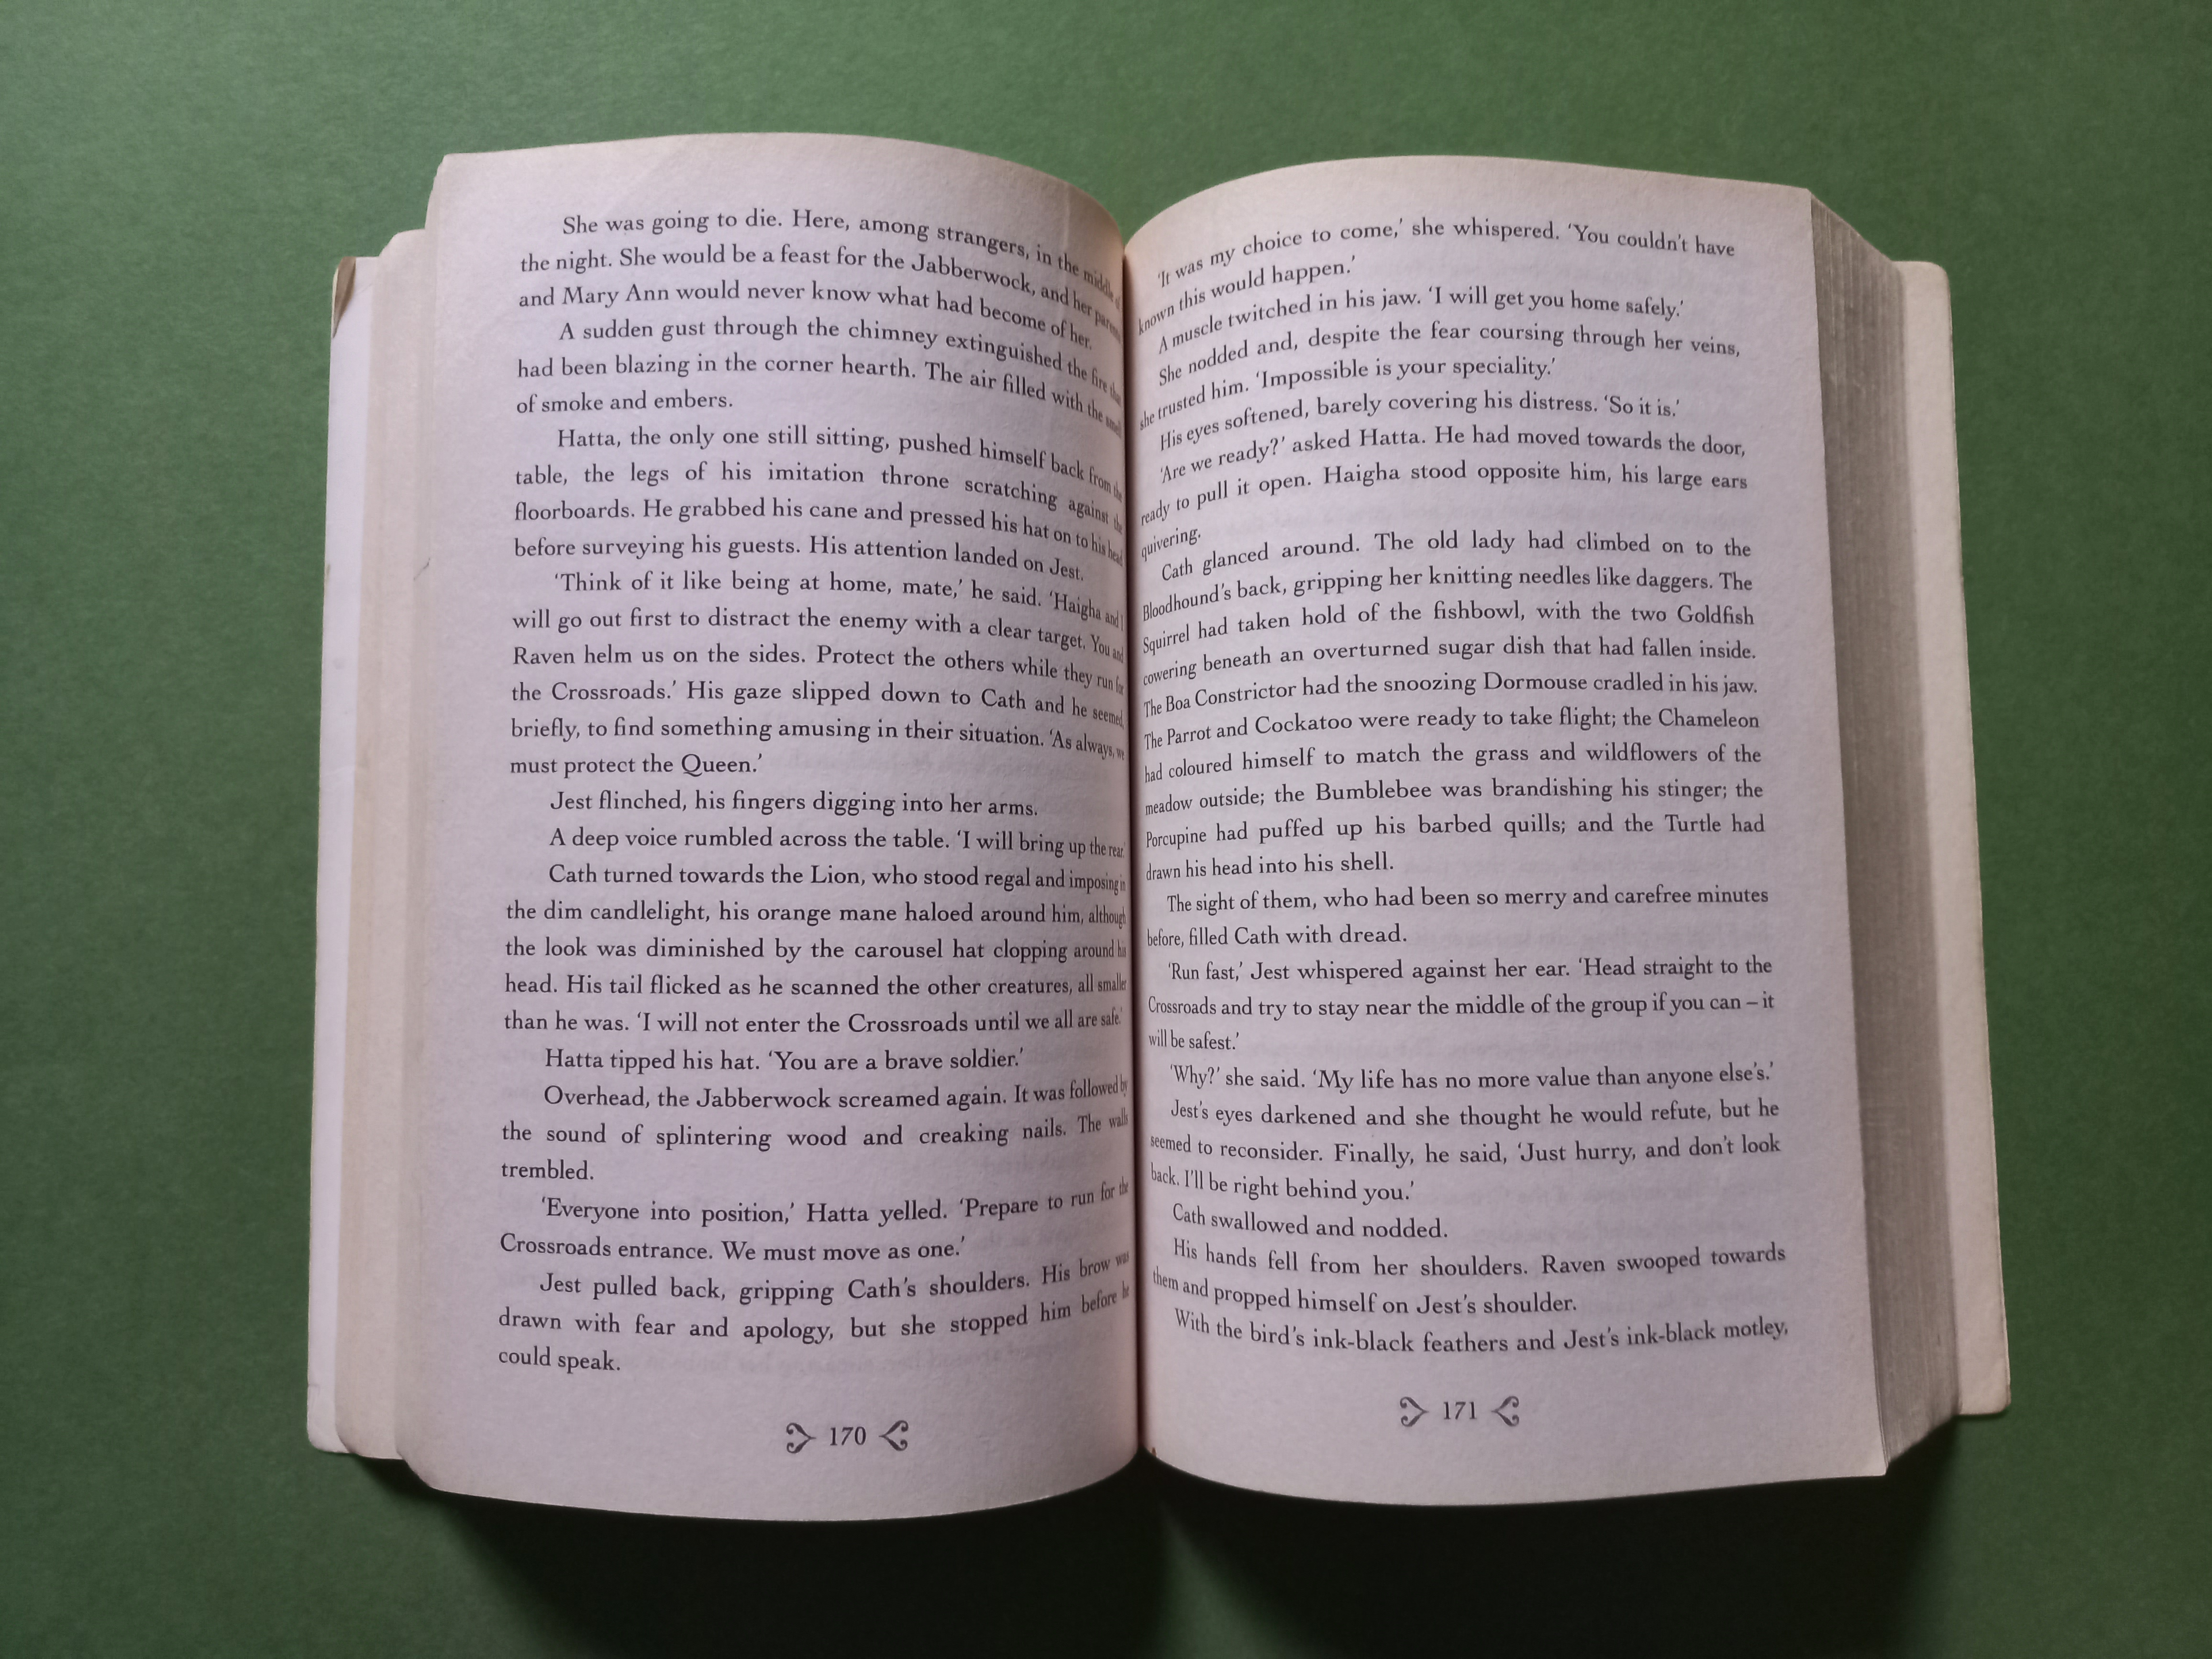
\includegraphics[width=4.0cm]{Figures/open_book.jpg}}
  %  \vspace{1.5cm}
    \centerline{(a) Input Image}\medskip
  \end{minipage}
  \hfill
  \begin{minipage}[b]{.48\linewidth}
    \centering
    \centerline{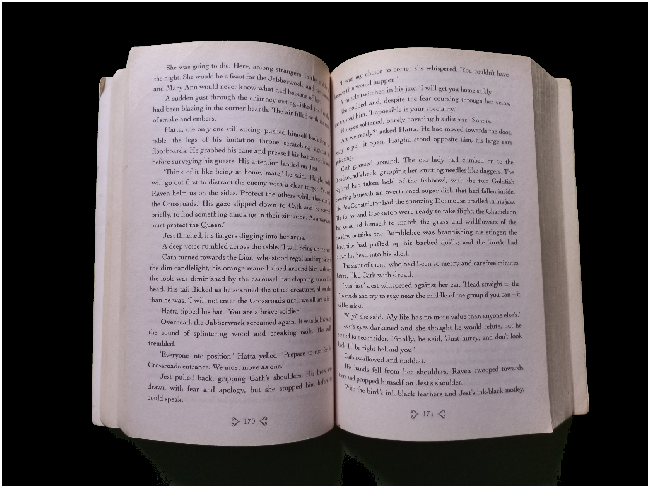
\includegraphics[width=4.0cm]{Figures/openbook_kmeans_result.png}}
  %  \vspace{1.5cm}
    \centerline{(b) K-Means}\medskip
  \end{minipage}
  \hfill
  \begin{minipage}[b]{0.48\linewidth}
    \centering
    \centerline{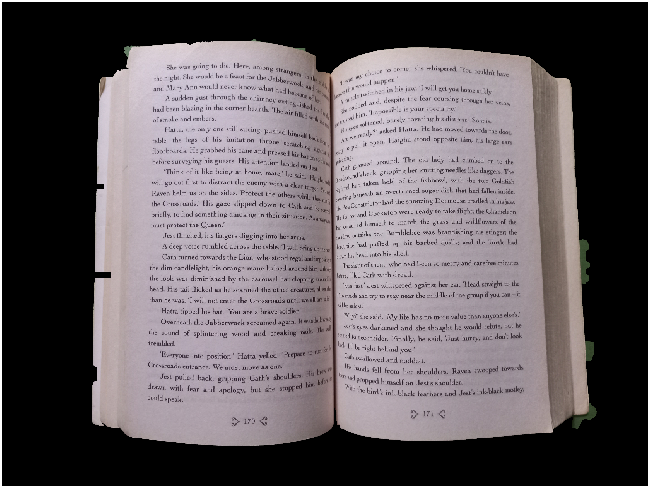
\includegraphics[width=4.0cm]{Figures/openbook_lazysnapping_result.png}}
  %  \vspace{1.5cm}
    \centerline{(c) Lazy Snapping}\medskip
  \end{minipage}
  %
  \hfill
  \begin{minipage}[b]{0.48\linewidth}
    \centering
    \centerline{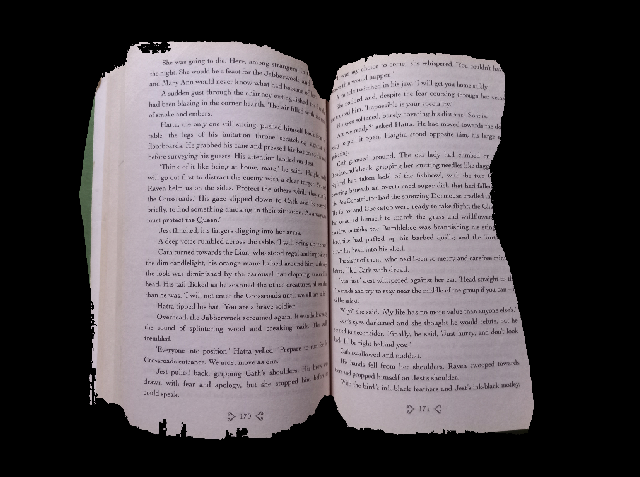
\includegraphics[width=4.0cm]{Figures/openbook_geodesic_result.png}}
  %  \vspace{1.5cm}
    \centerline{(d) Geodesic}\medskip
  \end{minipage}
  %
  \caption{Comparison of segmentation results using the three techniques.}
  \label{segmentation_res}
  %
\end{figure}

\subsection{Color Quantization Results}
\label{sec:quant_results}
Both quantization methods worked effectively and gave similar results in simplifying colors in the objects and giving them an illustrated effect. The book in Figure~\ref{segmentation_res} can be seen to have an illustrated effect after quantization in  Figure ~\ref{quantized_book}. Moreover, Figure ~\ref{quantized} shows more examples of input images and their illustrated versions. 

\begin{figure}[H]
  \begin{minipage}[b]{1.0\linewidth}
    \centering
    \centerline{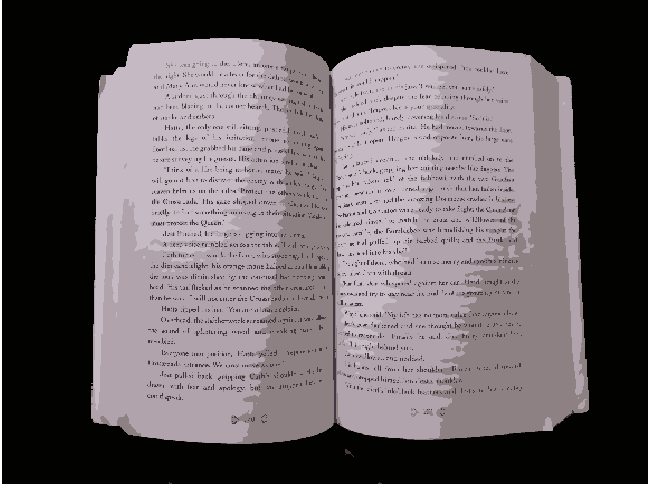
\includegraphics[width=8.0cm]{Figures/openbook_kmeans_quant.png}}
  %  \vspace{1.5cm}
    % \centerline{(a) Input Image}\medskip
  \end{minipage}
  \caption{Book image after quantization.}
  \label{quantized_book}
\end{figure}

\begin{figure}[H]
  \begin{minipage}[b]{1.0\linewidth}
    \centering
    \centerline{\includegraphics[width=8.0cm]{Figures/illustrated.png}}
  %  \vspace{1.5cm}
    % \centerline{(a) Input Image}\medskip
  \end{minipage}
  \caption{Left column: input images. Right column: segmented and color quantized.}
  \label{quantized}
\end{figure}

\subsection{Limitations and Future Directions}

A limitation of this implementation is that images must have a solid colored background with no other objects or colorful backgrounds in order for accurate segmentation to take place. Moreover, quantization of colors does give an illustrated effect but also eliminates detail which may in some cases include major parts of the object in question. 

Further work on this application can attempt to determine if a pattern exists between the nature of an image (illumination, background) and the most effective segmentation technique for it. That may allow us to group together input images and use the segmentation technique best suited to it. Moreover, the "illustrated" images produced in this implementation have sharp edges and real-world forms. In order to give a more illustrated look, perhaps methods of softening sharp edges and distorting proportions can be implemented as well. In addition, an effective coherent line drawing algorithm can also be implemented in order to enhance only the principle boundaries of illustrated objects for a more effective illustrated effect. 

\section{Conclusion}
\label{sec:conclusion}

This paper aimed to explore existing MATLAB algorithms/functions that may be used to extract objects from images and give them an illustrated effect for use in graphic design by smoothing (bilateral filter), extracting the object (segmentation), and color quantization. As can be seen in Figure~\ref{posters}, existing algorithms are capable of producing such illustrations. Further work on this application can look into various other illustrated effects and art styles that can be implemented, as well as implementing an edge detection and linking method to enhance the edges of the illustrations in a visually appealling manner.

\begin{figure}[H]
  \begin{minipage}[b]{1.0\linewidth}
    \centering
    \centerline{
\includegraphics[width=8.0cm]{Figures/posters2.png}}
  %  \vspace{1.5cm}
    % \centerline{(a) Input Image}\medskip
  \end{minipage}
  \caption{Posters made using illustrations generated in this project from smartphone-captured images.}
  \label{posters}
\end{figure}

% Below is an example of how to insert images. Delete the ``\vspace'' line,
% uncomment the preceding line ``\centerline...'' and replace ``imageX.ps''
% with a suitable PostScript file name.
% -------------------------------------------------------------------------
% \begin{figure}[htb]

% \begin{minipage}[b]{1.0\linewidth}
%   \centering
%   \centerline{\includegraphics[width=8.5cm]{Fig1.png}}
% %  \vspace{2.0cm}
%   \centerline{(a) Result 1}\medskip
% \end{minipage}
% %
% \begin{minipage}[b]{.48\linewidth}
%   \centering
%   \centerline{\includegraphics[width=4.0cm]{Fig3anew.png}}
% %  \vspace{1.5cm}
%   \centerline{(b) Results 3}\medskip
% \end{minipage}
% \hfill
% \begin{minipage}[b]{0.48\linewidth}
%   \centering
%   \centerline{\includegraphics[width=4.0cm]{Fig4new.png}}
% %  \vspace{1.5cm}
%   \centerline{(c) Result 4}\medskip
% \end{minipage}
% %
% \caption{Example of placing a figure with experimental results.}
% \label{fig:res}
% %
% \end{figure}

% To start a new column (but not a new page) and help balance the last-page
% column length use \vfill\pagebreak.
% -------------------------------------------------------------------------
\vfill
\pagebreak


% References should be produced using the bibtex program from suitable
% BiBTeX files (here: strings, refs, manuals). The IEEEbib.bst bibliography
% style file from IEEE produces unsorted bibliography list.
% -------------------------------------------------------------------------
\bibliographystyle{IEEEbib}
\bibliography{DIP_project}

\end{document}
